
\documentclass[conference]{IEEEtran}
\usepackage{balance}
\usepackage{moreverb}
\usepackage{amsmath}
\usepackage[utf8]{inputenc}
    \usepackage{listings}  
    \usepackage{color}  
    \usepackage{textcomp}  
    \definecolor{listinggray}{gray}{0.98}  
    \definecolor{lbcolor}{rgb}{0.98,0.98,0.98}  
    \lstset{  
     backgroundcolor=\color{lbcolor},  
     tabsize=4,  
     rulecolor=,  
     language=java,  
            basicstyle=\scriptsize,  
            upquote=true,  
            aboveskip={1.5\baselineskip},  
            columns=fixed,  
            showstringspaces=false,  
            extendedchars=true,  
            breaklines=true,  
            showtabs=false,  
            showspaces=false,  
            showstringspaces=false,  
            identifierstyle=\ttfamily,  
            keywordstyle=\color[rgb]{0,0,1},  
            commentstyle=\color[rgb]{0.133,0.545,0.133},  
            stringstyle=\color[rgb]{0.627,0.126,0.941},  
    }

\ifCLASSINFOpdf
   \usepackage[pdftex]{graphicx}
\else
\fi

\addtolength{\textwidth}{2mm}
\hyphenation{op-tical net-works semi-conduc-tor}

\begin{document}
\title{Data Synchronization and Replication Tool}

\author{\IEEEauthorblockN{Pradeeban Kathiravelu}
\IEEEauthorblockA{INESC-ID Lisboa\\
Instituto Superior T\'{e}cnico, Universidade de Lisboa\\
Lisbon, Portugal\\
Email: pradeeban.kathiravelu@tecnico.ulisboa.pt}
\and
\IEEEauthorblockN{Ashish Sharma}
\IEEEauthorblockA{Department of Biomedical Informatics\\
Emory University\\
Atlanta, Georgia, USA\\
Email: ashish.sharma@emory.edu}}
\maketitle

\begin{abstract}
Consumers download the data by searching the image repository using the browser. The information that the consumer is interested in, gets updated whenever the data producers update or add patient information. The current download tool lacks the ability to track the relevant updates to the consumer. A data replication and synchronization tool will assist automated downloads to the consumers.
\end{abstract}

\IEEEpeerreviewmaketitle

\section{Introduction}
\section{Background}
Medical images are represented in multiple granularity. Figure~\ref{fig:granularity} represents how the images are structured hierarchically in TCIA.
\begin{figure}[ht]
\begin{center}
 \resizebox{\columnwidth}{!}{
  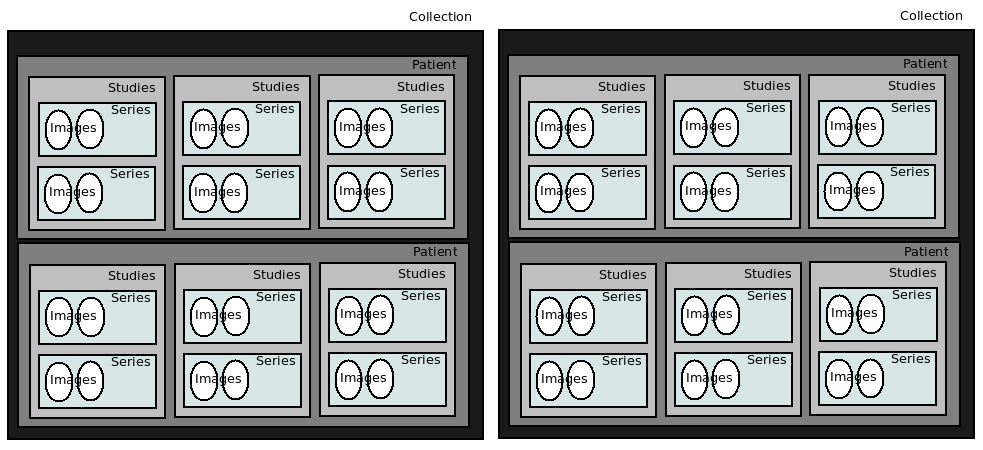
\includegraphics[width=\textwidth]{tcia.png}
 }
\end{center}
 \caption{Medical Images Granularity}
 \label{fig:granularity}
\end{figure}

\section{Design and Implementation}
\subsection{Deployment}
Having multiple instances running over different nodes provide fault-tolerance, as when one node terminates, the other nodes have the backup replica of the partitions stored in the terminated node. Figure~\ref{fig:deployment} shows the higher level deployment view of the solution.
\begin{figure}[ht]
\begin{center}
 \resizebox{0.6\columnwidth}{!}{
  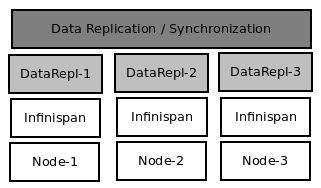
\includegraphics[width=0.6\textwidth]{deployment.png}
 }
\end{center}
 \caption{Deployment}
 \label{fig:deployment}
\end{figure}

\subsection{Design}
Two distributed cache instances exist in InfDataAccessIntegration.
\begin{lstlisting}  
    protected static Cache userReplicasMap;
    protected static Cache replicaSetsMap;
\end{lstlisting}  
userReplicasMap is a mapping of userId -> Array of replicaSetIDs. UserID could be the logged in user name. (for now, testing with random strings).
replicaSetsMap is a mapping of replicaSetID -> replicaSet

Though this could be replaced with a single cache instance with the mapping of userID -> replicaSets, having two cache instances will be more efficient during searches, duplicates, and push changes. Hence, two cache instances design was chosen.

$InfDataAccessIntegration$ provides the API for publisher/consumer, $TCIAInvoker$ which extends the abstract class InterfaceManager, implements the TCIA integration to invoke these methods. Figure~\ref{fig:class} provides a core class hierarchy of the system.
\begin{figure}[ht]
\begin{center}
 \resizebox{0.6\columnwidth}{!}{
  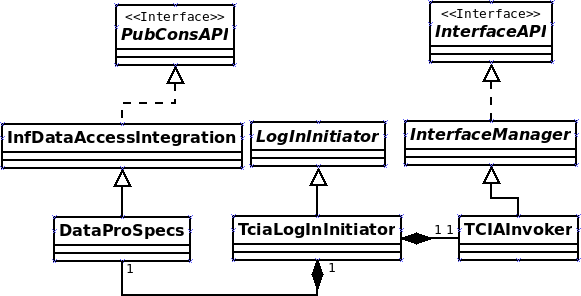
\includegraphics[width=0.6\textwidth]{classDiagram.png}
 }
\end{center}
 \caption{Core Class Hierarchy}
 \label{fig:class}
\end{figure}

\subsection{Execution Flow}
The execution flow is depicted by Figure~\ref{fig:execution}. When the user logs in, $logIn()$ checks whether the user has already stored replicaSets from the Infinispan distributed Cache. If so, execute them all again. This would be changed later as we do not have to execute all. Rather, we need to execute for the diffs. When the user performs new searches, for the images, series, collections, and the other meta data, the results will be returned to the user, and the user can chose ta subset of the returned results to create a replicaSet.
\begin{figure}[ht]
\begin{center}
 \resizebox{\columnwidth}{!}{
  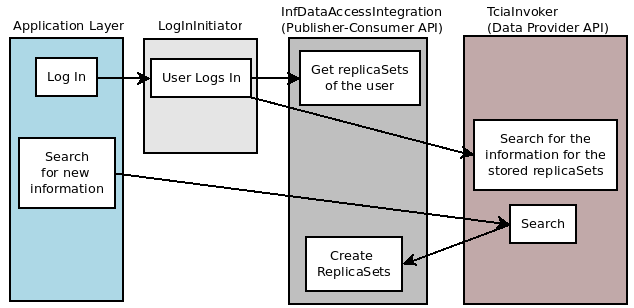
\includegraphics[width=\textwidth]{execFlow.png}
 }
\end{center}
 \caption{Execution Flow}
 \label{fig:execution}
\end{figure}
The replicaSet for the image will be as,
\begin{lstlisting}  
TCIAConstants.IMAGE_TAG + "getImage?SeriesInstanceUID=" + seriesInstanceUID
\end{lstlisting}  
For other information (meta data), such as collections and seies,
\begin{lstlisting}  
TCIAConstants.META_TAG + query;
Here, query is something like, "getSeries?format=" + format +
                "&Collection=" + collection +
                "&PatientID=" + patientID +
                "&StudyInstanceUID=" + studyInstanceUID +
                "&Modality=" + modality;
\end{lstlisting}  
When a new instance starts now, and invokes the log in action for the same user, it will execute the queries for the stored replicaSets again, and reproduce the same results.
\section{Evaluation}
\section{Conclusion}
\balance

%\begin{thebibliography}{1}
%\end{thebibliography}

\end{document}
